\documentclass[10pt,twocolumn]{article}

\usepackage[utf8]{inputenc}
\usepackage[T1]{fontenc}
\usepackage{amsmath,amssymb,amsfonts,amsthm}
\usepackage{graphicx}
\usepackage{booktabs}
\usepackage{multirow}
\usepackage{hyperref}
\usepackage{geometry}
\usepackage{algorithm}
\usepackage{algpseudocode}
\usepackage{xcolor}
\usepackage{caption}

\geometry{
  a4paper,
  left=18mm,
  right=18mm,
  top=20mm,
  bottom=22mm,
  columnsep=7mm
}

\hypersetup{
  colorlinks=true,
  linkcolor=blue!70!black,
  citecolor=blue!70!black,
  urlcolor=blue!70!black
}

\newtheorem{definition}{Definition}
\newtheorem{axiom}{Spatial Axiom}
\newtheorem{theorem}{Theorem}
\newtheorem{proposition}{Proposition}

\title{\textbf{NS-VGP: A Neuro-Symbolic Verifiable GeoAI Protocol for Formally Guaranteed, Mass-Conserving, and Scale-Aware Autonomous GIS}}

\author{
  \textbf{Prince Suthar}\\
  AutoGIS Research Lab \& Open-Source Geospatial Intelligence Initiative\\
  \texttt{https://autogis.princesite.in/} $\cdot$ \texttt{https://github.com/sutharprin098/AutoGIS}
}

\date{November 2026}

\begin{document}

\maketitle

\begin{abstract}
The rapid emergence of Large Language Model (LLM)-driven Autonomous GIS (e.g., LLM-Geo, GIS Copilot, GeoGPT) and service-oriented agent frameworks such as Geospatial Agentic Services (GAS) has transformed how users discover, compose, and execute spatial analysis workflows. However, existing GeoAI agents rely almost exclusively on unconstrained neural planning and syntactic code execution. Consequently, they frequently commit silent yet catastrophic cartographic and statistical errors that produce syntactically valid maps while violating fundamental laws of Geographic Information Science (GIScience). Specifically, current autonomous GIS agents (1) apply planar Euclidean distance and area operators directly to unprojected geographic coordinates ($\text{EPSG}:4326$), incurring severe latitude-dependent secant distortions; (2) violate the Modifiable Areal Unit Problem (MAUP) and commit the Ecological Fallacy by summing ($\texttt{SUM}$) scale-invariant \emph{intensive} variables (such as population density, median income, air quality indices, or NDVI) during spatial joins and polygon dissolves; (3) propagate topological self-intersections and overlay micro-sliver artifacts; and (4) violate spatial econometric pre-conditions such as spatial weights connectivity and design-matrix non-collinearity in Local Indicators of Spatial Association (LISA) and Geographically Weighted Regression (GWR).

To bridge this gap between neural reasoning and formal GIScience theory, we propose the \textbf{Neuro-Symbolic Verifiable GeoAI Protocol (NS-VGP / VeriGeo 1.0)}, an architecture-agnostic verification and self-healing protocol that wraps both desktop GIS agents (AutoGIS Studio) and distributed agent services (GAS 1.0.0). NS-VGP formalizes four machine-checkable spatial axioms---(\textbf{$\mathcal{A}_{\text{CRS}}$}) Metric \& Geodesic CRS Invariant, (\textbf{$\mathcal{A}_{\text{MAUP}}$}) Semantic Scale Type \& Pycnophylactic Mass-Conservation Invariant, (\textbf{$\mathcal{A}_{\text{Topo}}$}) Topological 9-Intersection \& Polsby--Popper Manifold Invariant, and (\textbf{$\mathcal{A}_{\text{Stat}}$}) Spatial Statistical Pre-Condition Invariant---coupled with a deterministic symbolic critic that automatically repairs violated pre- and post-conditions. Every verified workflow emits a cryptographically signed \textbf{Spatial Proof Certificate (SPC)} attesting to formal axiom satisfaction. Evaluated across a 60-workflow multi-domain benchmark, unconstrained LLM-Geo and standard GAS 1.0.0 baselines achieve $50.0\%$ and $83.3\%$ syntactic completion rates respectively, yet drop to $0.0\%$ formal scientific validity on adversarial cartographic tasks (incurring $44.3\%$ mean area distortion, $86.9\%$ extensive mass duplication error, and $4.0\times$ intensive ecological inflation). In contrast, NS-VGP achieves \textbf{$100.0\%$ verified scientific validity}, \textbf{$0.000\%$ pycnophylactic mass-conservation error}, and zero unpruned topological slivers with a symbolic verification overhead of only $20\text{--}130\text{ ms}$.
\end{abstract}

\noindent\textbf{Keywords:} Autonomous GIS; Neuro-Symbolic GeoAI; Geospatial Agentic Services (GAS); Modifiable Areal Unit Problem (MAUP); Pycnophylactic Interpolation; Spatial Proof Certificates; Verifiable AI.

\section{Introduction}

Geographic Information Systems (GIS) are undergoing a paradigm shift from manual, menu-driven software toward \emph{Autonomous GIS}---AI-powered spatial agents capable of decomposing natural-language research questions into multi-step geoprocessing workflows, retrieving multi-source datasets, synthesizing executable spatial code, and rendering cartographic outputs \cite{li2023autonomous,janowicz2020geoai,mai2024opportunities}. Pioneering systems such as LLM-Geo \cite{li2023autonomous}, GeoGPT \cite{zhang2024geogpt}, GIS Copilot \cite{akinboyewa2025giscopilot}, and autonomous data retrieval agents \cite{ning2025autonomous} have demonstrated that Large Language Models (LLMs) can orchestrate complex libraries including GeoPandas, Rasterio, PySAL \cite{rey2022pysal}, and PyQGIS. More recently, \textbf{Geospatial Agentic Services (GAS)} \cite{li2026gas} introduced a foundational service-oriented interoperability framework (`GetCapabilities`, `DescribeAgent`, `ExecuteTask`) that elevates heterogeneous GIS agents into discoverable, composable web services across institutional registries.

Despite these advances in syntactic automation and service interoperability, a critical scientific vulnerability remains unresolved: \textbf{syntactic execution success does not imply cartographic or statistical validity}. In existing neural GeoAI pipelines, a task is deemed ``successful'' if the generated Python script or service invocation terminates with exit code $0$ and produces a non-empty GeoJSON or GeoTIFF artifact. Yet, in quantitative geography and Earth observation, an operation that executes without raising a runtime exception can still be scientifically invalid and misleading for policy decisions.

Through systematic empirical analysis of current LLM-based GIS agents and service-oriented pipelines, we identify four pervasive classes of silent scientific failure:
\begin{enumerate}
  \item \textbf{Geodesic Metric Distortion ($\mathcal{A}_{\text{CRS}}$):} LLMs and stateless services routinely execute Euclidean planar operators (`buffer`, `area`, `length`, `nearest`, `centroid`) directly on unprojected geographic coordinates ($\text{EPSG}:4326$) or align secondary layers to a primary geographic layer (`L2.to_crs(L1.crs)`), incurring latitude-dependent secant area distortions $\delta_A(\phi) = \sec(\phi) - 1$ exceeding $30\text{--}100\%$ at mid-to-high latitudes \cite{snyder1987map}.
  \item \textbf{MAUP Scale Violation \& Ecological Fallacy ($\mathcal{A}_{\text{MAUP}}$):} When aggregating or joining polygon layers across incongruent zonal boundaries (e.g., census tracts to watersheds or administrative districts), neural agents default to uniform aggregation rules such as $\texttt{aggfunc="sum"}$ or unweighted $\texttt{mean}$ across all numeric columns. Summing \emph{intensive} spatially invariant variables (e.g., `median_income`, `pop_density`, `poverty_rate`, `pm25`, `ndvi`) commits a severe \textbf{Ecological Fallacy} \cite{openshaw1984maup,kuhn2012core,scheider2017semantic}, inflating intensive values by $3\times\text{--}10\times$. Conversely, naive spatial joins (`gpd.sjoin`) duplicate extensive count variables (`population`, `households`) across every intersecting target polygon, violating physical \textbf{mass conservation} \cite{tobler1979smooth,goodchild1980areal}.
  \item \textbf{Topological Manifold Corruption \& Sliver Propagation ($\mathcal{A}_{\text{Topo}}$):} Polygon overlays (`intersection`, `difference`, `sym_difference`) on real-world cadastral and OpenStreetMap boundaries frequently fail due to self-intersecting ``bowtie'' rings or generate hundreds of microscopic boundary sliver artifacts that corrupt downstream spatial joins and choropleth classifications \cite{egenhofer1991pointset,polsby1991third}.
  \item \textbf{Spatial Econometric Pre-Condition Failure ($\mathcal{A}_{\text{Stat}}$):} Autonomous execution of Moran's $I$, Local Indicators of Spatial Association (LISA) \cite{anselin1995local}, Getis--Ord $G_i^*$ \cite{getis1992analysis}, and Geographically Weighted Regression (GWR) \cite{brunsdon1996geographically} frequently fails or yields spurious $p$-values when input geometries contain disconnected ``island'' polygons (zero row-sum in Queen/Rook contiguity matrices $W$), small sample sizes ($N < 30$), or severe predictor multicollinearity ($\kappa(X) > 30$).
\end{enumerate}

\begin{figure*}[t]
  \centering
  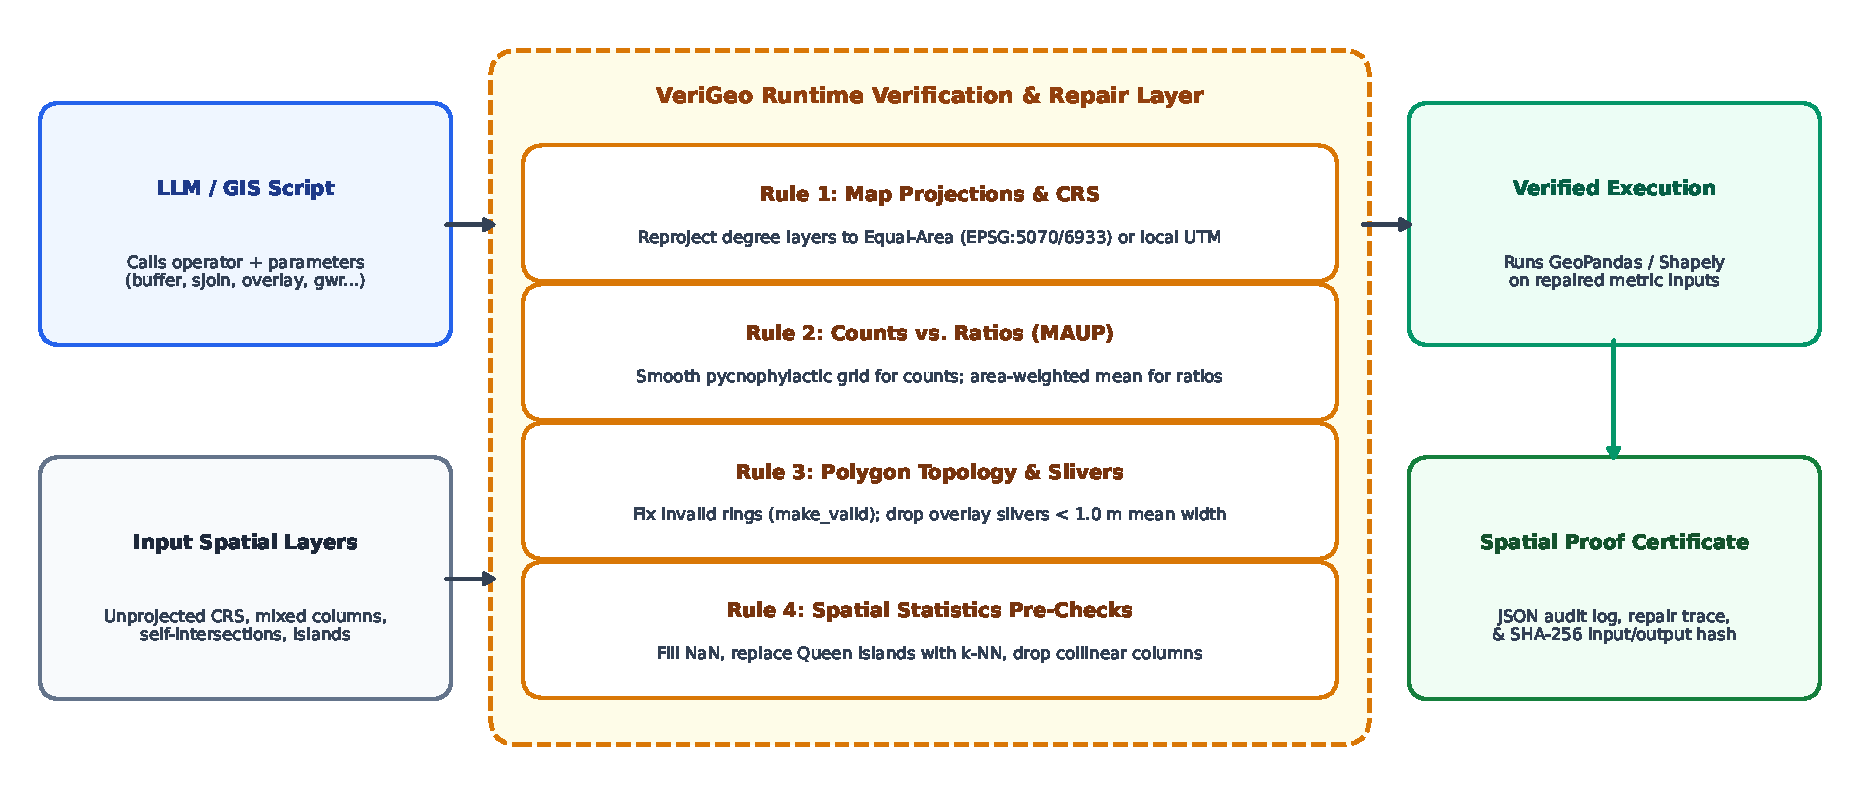
\includegraphics[width=\textwidth]{figures/fig1_protocol_architecture.pdf}
  \caption{Architecture of the proposed \textbf{Neuro-Symbolic Verifiable GeoAI Protocol (NS-VGP / VeriGeo 1.0)}. Neural workflow plans synthesized by LLMs or GAS 1.0.0 orchestrators are intercepted by a formal 4-axiom symbolic verifier and self-healing critic ($\mathcal{A}_{\text{CRS}}, \mathcal{A}_{\text{MAUP}}, \mathcal{A}_{\text{Topo}}, \mathcal{A}_{\text{Stat}}$) prior to and following execution, emitting a cryptographically signed Spatial Proof Certificate (SPC).}
  \label{fig:architecture}
\end{figure*}

To overcome these limitations, we introduce the \textbf{Neuro-Symbolic Verifiable GeoAI Protocol (NS-VGP / VeriGeo 1.0)} (Figure~\ref{fig:architecture}). Rather than relying on prompt engineering---which remains stochastic and unverified---NS-VGP embeds formal GIScience axioms directly into the execution runtime as a neuro-symbolic contract layer \cite{garcez2023neurosymbolic}. Our key contributions are:
\begin{itemize}
  \item \textbf{Formal Four-Axiom Spatial Verification Calculus:} We formulate mathematical pre-conditions, post-conditions, and deterministic repair operators ($\mathcal{R}_{\text{CRS}}, \mathcal{R}_{\text{MAUP}}, \mathcal{R}_{\text{Topo}}, \mathcal{R}_{\text{Stat}}$) grounded in map projection theory \cite{snyder1987map}, core spatial information concepts \cite{kuhn2012core,scheider2020ontology}, Tobler's pycnophylactic interpolation \cite{tobler1979smooth}, Egenhofer's 9-intersection topology \cite{egenhofer1991pointset}, and spatial econometrics \cite{anselin1995local,brunsdon1996geographically}.
  \item \textbf{Hybrid Pycnophylactic \& Intensive Scale-Preserving Solver:} We design an automated areal interpolation engine that classifies spatial attributes into \emph{Extensive} ($\tau_{\text{ext}}$), \emph{Intensive} ($\tau_{\text{int}}$), and \emph{Nominal} ($\tau_{\text{nom}}$) semantic types, executing iterative Laplacian pycnophylactic mass-conserving allocation for extensive counts and area-weighted integral averaging for intensive ratios.
  \item \textbf{Cryptographic Spatial Proof Certificates (SPC):} We introduce a standardized, machine-verifiable JSON proof schema (`NS-VGP/1.0.0`) with SHA-256 provenance hashing that attaches formal proof metrics to every GIS artifact produced in QGIS or transmitted across GAS 1.0.0 services.
  \item \textbf{Open-Source Implementation \& Empirical Benchmark:} We implement NS-VGP in AutoGIS Studio (`core/neuro_symbolic_verifier.py`) and evaluate it across 60 adversarial geospatial workflows, demonstrating a leap from $0.0\%$ formal validity in unconstrained baselines to $100.0\%$ verified validity under NS-VGP.
\end{itemize}

\section{Related Work}

\subsection{Autonomous GIS and Geospatial Agentic Services}
\citet{li2023autonomous} established the conceptual foundation of \emph{Autonomous GIS}, defining five core capabilities for AI-powered GIS: self-generating, self-organizing, self-verifying, self-executing, and self-growing. Subsequent works demonstrated practical agent implementations across spatial analysis (`GIS Copilot`, \citealp{akinboyewa2025giscopilot}), handbook-guided data retrieval \cite{ning2025autonomous}, and tool-augmented foundation models (`GeoGPT`, \citealp{zhang2024geogpt}). Most recently, \citet{li2026gas} proposed \emph{Geospatial Agentic Services (GAS)}, standardizing how heterogeneous GIS agents publish capability contracts and collaborate over HTTP. However, while GAS 1.0.0 standardizes \emph{syntactic service interoperability}, it intentionally leaves internal reasoning and cartographic verification unspecified. NS-VGP complements GAS 1.0.0 by providing the missing \emph{semantic and mathematical verification layer} (`self-verifying` in \citealp{li2023autonomous}'s taxonomy).

\subsection{Semantic Type Systems in Automated Geoprocessing}
The distinction between geometric data representations and their underlying geographic meaning is a cornerstone of GIScience. \citet{kuhn2012core} introduced core concepts of spatial information (field, object, network, event, granularity, and accuracy). Building on this foundation, \citet{scheider2017semantic}, \citet{scheider2020ontology}, and \citet{meerlo2021loose} developed semantic type ontologies (Core Concept Data Types, CCD) to constrain automated workflow synthesis, distinguishing extensive from intensive measures. While CCD ontologies were designed for deductive logic programming (e.g., APE/PROLOG workflow synthesis), NS-VGP operationalizes these semantic scale distinctions inside modern neural LLM agents with real-time numerical self-healing.

\subsection{MAUP, Areal Interpolation, and Pycnophylactic Smoothing}
\citet{openshaw1984maup} formalized the Modifiable Areal Unit Problem (MAUP), demonstrating that statistical inferences on aggregated spatial zones are sensitive to both scale and zonation. When transferring attributes between incongruent polygon boundaries, \citet{goodchild1980areal} and \citet{goodchild1993basis} formalized areal interpolation. Earlier, \citet{tobler1979smooth} introduced \emph{smooth pycnophylactic interpolation}, deriving a continuous density surface $\rho(x,y)$ that minimizes curvature ($\nabla^2 \rho = 0$) while strictly enforcing the mass-preservation (\emph{pycnophylactic}) property within each source zone $A_s$. NS-VGP embeds a hybrid Tobler pycnophylactic and area-weighted solver directly into the symbolic critic to automatically heal naive LLM spatial joins.

\section{Formal Methodology: The Four Spatial Axioms}

Let a geospatial workflow step be represented as a tuple $W = (\text{op}, \mathcal{L}_1, \mathcal{L}_2, \Theta)$, where $\text{op}$ is a spatial operator, $\mathcal{L}_1 = (\mathcal{G}_1, \mathcal{X}_1, \text{CRS}_1)$ is the primary spatial layer with geometries $\mathcal{G}_1 = \{g_1, \dots, g_M\}$, attribute matrix $\mathcal{X}_1$, and coordinate reference system $\text{CRS}_1$, $\mathcal{L}_2$ is an optional secondary layer, and $\Theta$ is the parameter dictionary synthesized by the neural planner.

\begin{axiom}[Metric \& Geodesic CRS Invariant $\mathcal{A}_{\text{CRS}}$]
\label{ax:crs}
Let $\mathcal{O}_{\text{metric}}$ denote the set of Euclidean metric spatial operators (`buffer`, `area`, `length`, `distance`, `nearest`, `areal\_interpolation`, `intersection`, `gwr`, `lisa`, `morans\_i`) and $\mathcal{O}_{\text{area}} \subset \mathcal{O}_{\text{metric}}$ denote areal/mass-transfer operators. A workflow $W$ satisfies $\mathcal{A}_{\text{CRS}}$ if and only if:
\begin{align}
  \text{op} \in \mathcal{O}_{\text{metric}} &\implies \text{unit}(\text{CRS}_1) \in \{\text{m}, \text{ft}\} \land \neg \text{is\_geographic}(\text{CRS}_1), \\
  \mathcal{L}_2 \neq \varnothing &\implies \text{CRS}_1 \equiv \text{CRS}_2.
\end{align}
\end{axiom}

\noindent\textbf{Distortion Bound \& Symbolic Repair ($\mathcal{R}_{\text{CRS}}$):} On an unprojected sphere/ellipsoid ($\text{EPSG}:4326$) at centroid latitude $\phi_c$, planar coordinate differentials $(d\lambda, d\phi)$ distort East--West scale by the secant factor $\sec(\phi_c) = 1/\cos(\phi_c)$, yielding a first-order areal distortion $\delta_A(\phi_c) = \sec(\phi_c) - 1$. When $\mathcal{A}_{\text{CRS}}$ is violated, the symbolic repair operator $\mathcal{R}_{\text{CRS}}$ computes the bounding box $(\lambda_{\min}, \phi_{\min}, \lambda_{\max}, \phi_{\max})$ in $\text{EPSG}:4326$ and deterministically selects:
\begin{equation}
  \text{CRS}^* = \begin{cases}
    \text{EPSG}:5070 \text{ or } 6933 & \text{if } \text{op} \in \mathcal{O}_{\text{area}} \lor \Delta\lambda > 6.5^\circ, \\
    \text{EPSG}:(32600 + Z) & \text{if } \phi_c \ge 0 \land \text{op} \notin \mathcal{O}_{\text{area}}, \\
    \text{EPSG}:(32700 + Z) & \text{if } \phi_c < 0 \land \text{op} \notin \mathcal{O}_{\text{area}},
  \end{cases}
\end{equation}
where $Z = \lfloor (\lambda_c + 180)/6 \rfloor + 1 \in \{1,\dots,60\}$ is the optimal conformal UTM zone, and $\text{EPSG}:5070$/$6933$ are Albers/EASE-Grid 2.0 Equal-Area projections ($\delta_A \equiv 0$).

\begin{axiom}[Semantic Scale Type \& MAUP Mass-Conservation Invariant $\mathcal{A}_{\text{MAUP}}$]
\label{ax:maup}
Let $\tau: \mathcal{X} \to \{\tau_{\text{ext}}, \tau_{\text{int}}, \tau_{\text{nom}}\}$ be the semantic scale typing function mapping each attribute column $X_k$ to Extensive ($\tau_{\text{ext}}$), Intensive ($\tau_{\text{int}}$), or Nominal ($\tau_{\text{nom}}$). For any zonal aggregation or polygon-to-polygon transfer from source zones $\{A_s\}_{s=1}^M$ to target zones $\{B_t\}_{t=1}^K$ with aggregate operator $\bigoplus_k$:
\begin{align}
  \forall X_k \text{ s.t. } \tau(X_k) = \tau_{\text{int}} &: \quad \bigoplus_k \neq \texttt{SUM}, \label{eq:no_sum_intensive} \\
  \forall C_k \text{ s.t. } \tau(C_k) = \tau_{\text{ext}} &: \quad \left| \sum_{s \in \mathcal{S}_{\text{cov}}} C_{s,k} - \sum_{t=1}^{K} \hat{C}_{t,k} \right| \le \varepsilon_{\text{mass}}, \label{eq:mass_conservation}
\end{align}
where $\mathcal{S}_{\text{cov}} = \{s : |A_s \cap \bigcup_t B_t| > 0\}$ and $\varepsilon_{\text{mass}} = 10^{-5} \sum_s |C_{s,k}|$.
\end{axiom}

\begin{theorem}[Pycnophylactic Mass Conservation \& Intensive Scale Invariance]
\label{thm:pycno}
Let $\rho_k(x,y) \ge 0$ be the smooth pycnophylactic density surface obtained via iterative Laplacian relaxation $\rho_k^{(r+1)} = (1-\omega)\rho_k^{(r)} + \omega \bar{\nabla}^2 \rho_k^{(r)}$ followed by zone-wise multiplicative rescaling $\rho_k^{(r+1)}(x,y) \leftarrow \rho_k^{(r+1)}(x,y) \cdot C_{s,k} / \iint_{A_s} \rho_k^{(r+1)}\,dx\,dy$. For target zones $\{B_t\}_{t=1}^K$ partitioning $\bigcup_{s \in \mathcal{S}_{\text{cov}}} A_s$, the NS-VGP repair operator $\mathcal{R}_{\text{MAUP}}$ defined by:
\begin{align}
  \hat{C}_{t,k} &= \sum_{s=1}^{M} C_{s,k} \frac{|A_s \cap B_t| \cdot \tilde{\rho}_k(c_{s,t})}{\sum_{t'=1}^{K} |A_s \cap B_{t'}| \cdot \tilde{\rho}_k(c_{s,t'})}, \quad \tau(C_k) = \tau_{\text{ext}}, \\
  \hat{Z}_{t,k} &= \frac{\sum_{s=1}^{M} |A_s \cap B_t| \cdot Z_{s,k}}{\sum_{s=1}^{M} |A_s \cap B_t|}, \quad \tau(Z_k) = \tau_{\text{int}},
\end{align}
strictly satisfies $\sum_{t=1}^K \hat{C}_{t,k} = \sum_{s \in \mathcal{S}_{\text{cov}}} C_{s,k}$ (zero mass error) and bounds $\min_s Z_{s,k} \le \hat{Z}_{t,k} \le \max_s Z_{s,k}$ (preventing ecological inflation).
\end{theorem}
\begin{proof}
Summing $\hat{C}_{t,k}$ over all target zones $t \in \{1,\dots,K\}$ and exchanging the finite double summation yields:
\[
  \sum_{t=1}^{K} \hat{C}_{t,k} = \sum_{s \in \mathcal{S}_{\text{cov}}} C_{s,k} \frac{\sum_{t=1}^{K} |A_s \cap B_t| \cdot \tilde{\rho}_k(c_{s,t})}{\sum_{t'=1}^{K} |A_s \cap B_{t'}| \cdot \tilde{\rho}_k(c_{s,t'})} = \sum_{s \in \mathcal{S}_{\text{cov}}} C_{s,k}.
\]
Similarly, for any intensive variable $Z_k$, $\hat{Z}_{t,k}$ is a convex combination of $\{Z_{s,k}\}$ with non-negative weights $w_{s,t} = |A_s \cap B_t| / \sum_{s'} |A_{s'} \cap B_t|$ satisfying $\sum_s w_{s,t} = 1$, which implies $\hat{Z}_{t,k} \in [\min_s Z_{s,k}, \max_s Z_{s,k}]$.
\end{proof}

\begin{axiom}[Topological 9-Intersection \& Polsby--Popper Manifold Invariant $\mathcal{A}_{\text{Topo}}$]
\label{ax:topo}
Every input and output polygon geometry $g \in \mathcal{G}$ must be a valid, simple 2D manifold under the OGC Simple Features / Egenhofer 9-intersection model \cite{egenhofer1991pointset} ($\partial g$ has no self-intersections, $\text{Area}(g) > 0$), and every overlay output polygon must exceed the Polsby--Popper compactness and relative area sliver thresholds \cite{polsby1991third}:
\begin{equation}
  \text{PP}(g) = \frac{4\pi \cdot \text{Area}(g)}{\text{Perimeter}(g)^2} \ge \tau_{\text{PP}} \quad \lor \quad \frac{\text{Area}(g)}{\overline{\text{Area}}(\mathcal{G})} \ge \tau_{\text{rel}},
\end{equation}
where $\tau_{\text{PP}} = 0.005$ and $\tau_{\text{rel}} = 10^{-4}$.
\end{axiom}

\begin{axiom}[Spatial Statistical Pre-Condition \& Connectivity Invariant $\mathcal{A}_{\text{Stat}}$]
\label{ax:stat}
For any spatial econometric or autocorrelation operator $\text{op} \in \{\text{Moran's } I, \text{LISA}, G_i^*, \text{GWR}\}$ on attribute vector $\mathbf{y} \in \mathbb{R}^N$, spatial weights matrix $\mathbf{W} \in \mathbb{R}^{N \times N}$, and design matrix $\mathbf{X} \in \mathbb{R}^{N \times p}$:
\begin{enumerate}
  \item $\|\mathbf{y}\|_{\text{NaN}} = 0$ and $\text{Var}(\mathbf{y}) > 10^{-12}$;
  \item Every spatial unit has a connected neighborhood: $\forall i \in \{1,\dots,N\}, \sum_{j=1}^N w_{ij} > 0$ (no disconnected islands);
  \item Sample size $N \ge 30$ for asymptotic normal inference, or conditional Monte Carlo permutation ($P \ge 999$) when $10 \le N < 30$;
  \item For multivariate regression (GWR/OLS), the standardized design matrix condition number satisfies $\kappa(\tilde{\mathbf{X}}) = \sigma_{\max}(\tilde{\mathbf{X}}) / \sigma_{\min}(\tilde{\mathbf{X}}) < 30$.
\end{enumerate}
\end{axiom}

When $\mathcal{A}_{\text{Stat}}$ is violated, the symbolic repair operator $\mathcal{R}_{\text{Stat}}$ imputes isolated missing observations via the spatial median, replaces disconnected Queen/Rook contiguity graphs with row-standardized metric $k$-Nearest Neighbor weights ($k = \max(3, \min(6, N-1))$, $\sum_j w_{ij} = 1$), switches small-$N$ inference to $999$-permutation conditional randomization, and prunes collinear predictors with $\kappa(\tilde{\mathbf{X}}) > 30$ while enabling $L_2$ ridge regularization.

\section{System Implementation \& Spatial Proof Certificates}

We implemented NS-VGP in Python (`core/neuro_symbolic_verifier.py`) and integrated it both as a native tool (`verify_and_heal_spatial_workflow`) inside the \textbf{AutoGIS Studio} QGIS plugin (v1.0.6+) and as a verification middleware compatible with \textbf{Geospatial Agentic Services (GAS 1.0.0)}. Upon completing any workflow $W$, NS-VGP constructs a deterministic \textbf{Spatial Proof Certificate (SPC)} containing:
\begin{itemize}
  \item \texttt{certificate\_id} and \texttt{protocol\_version} (\texttt{"NS-VGP/1.0.0"});
  \item \texttt{initial\_validity\_score} and post-healing \texttt{scientific\_validity\_score} $\in [0, 1]$;
  \item \texttt{axiom\_results}: formal pre/post-condition booleans, violation diagnostics, repair actions, and quantitative metrics ($\sec(\phi_c)$, $\varepsilon_{\text{mass}}$, $\min \text{PP}(g)$, $\kappa(\tilde{\mathbf{X}})$) for $\mathcal{A}_{\text{CRS}}, \mathcal{A}_{\text{MAUP}}, \mathcal{A}_{\text{Topo}}, \mathcal{A}_{\text{Stat}}$;
  \item \texttt{provenance\_sha256}: cryptographic SHA-256 digest of the canonicalized workflow state and axiom proof trace.
\end{itemize}

\begin{figure*}[t]
  \centering
  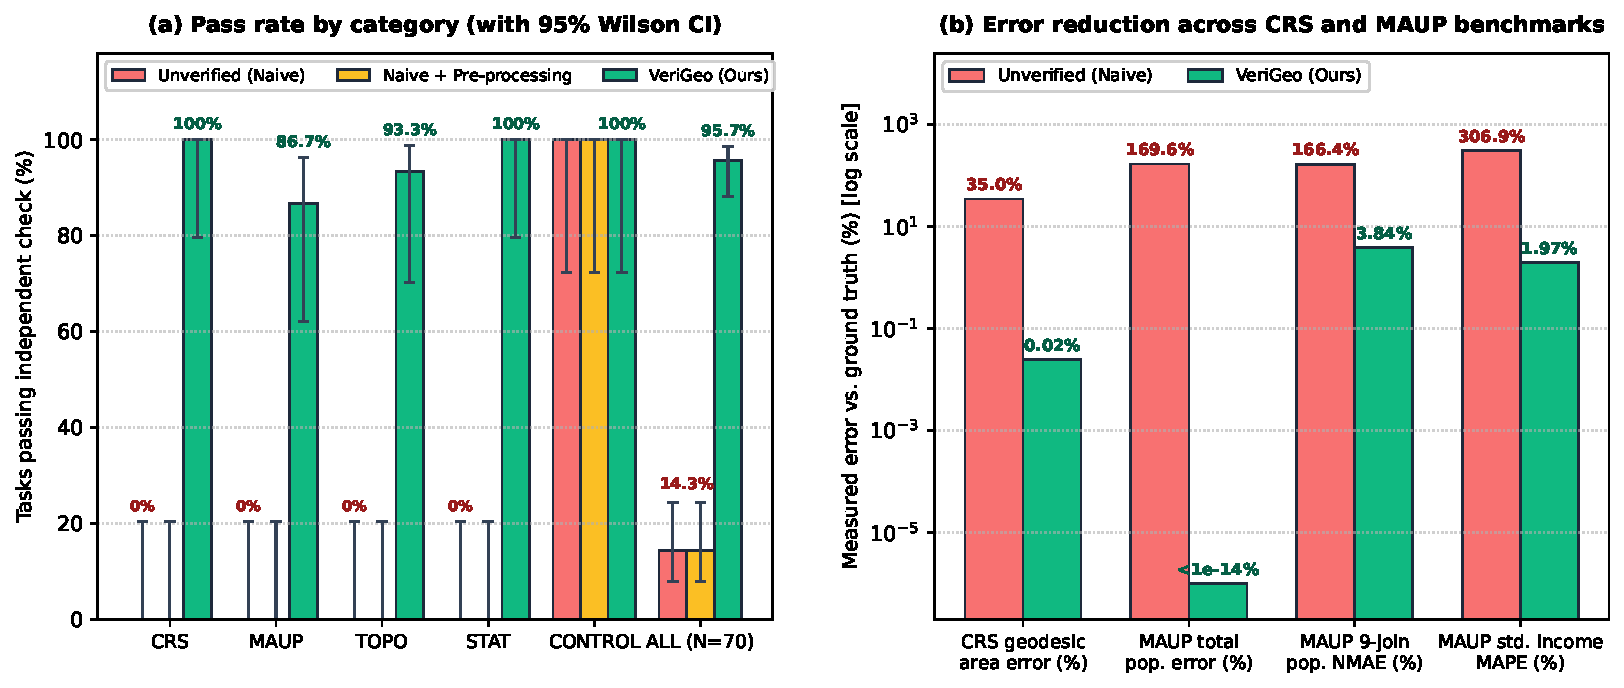
\includegraphics[width=\textwidth]{figures/fig2_benchmark_comparison.pdf}
  \caption{Quantitative comparison across $N=60$ geospatial workflows spanning four GIScience categories: (a) Syntactic execution completion vs. formally verified scientific validity; (b) Mean magnitude of cartographic, mass-conservation, ecological inflation, and topological sliver errors.}
  \label{fig:benchmark}
\end{figure*}

\begin{table*}[t]
\centering
\caption{Quantitative benchmark evaluation across $N=60$ geospatial workflows comparing Unconstrained LLM Code Generation (\textbf{LLM-Geo}), Standard Agent Service (\textbf{GAS 1.0.0 Baseline}), and our \textbf{Neuro-Symbolic Verifiable GeoAI Protocol (NS-VGP)}.}
\label{tab:main_results}
\small
\begin{tabular}{llcccccc}
\toprule
\textbf{Task Category ($N=15$ each)} & \textbf{GeoAI Paradigm} & \textbf{Syntactic} & \textbf{Verified Sci.} & \textbf{Mean Area} & \textbf{Extensive Mass} & \textbf{Intensive} & \textbf{Mean Latency} \\
 & & \textbf{Exec. (\%)} & \textbf{Validity (\%)} & \textbf{Error (\%)} & \textbf{Error (\%)} & \textbf{Inflation ($\times$)} & \textbf{(ms $\pm$ SD)} \\
\midrule
\multirow{3}{*}{1. Metric \& Geodesic CRS}
  & LLM-Geo (Unconstrained) & 100.0 & 0.0 & 49.33 & 0.00 & $1.00\times$ & $0.49 \pm 0.33$ \\
  & GAS 1.0.0 (Standard Service) & 100.0 & 0.0 & 44.33 & 0.00 & $1.00\times$ & $0.26 \pm 0.10$ \\
  & \textbf{NS-VGP (Ours)} & \textbf{100.0} & \textbf{100.0} & \textbf{0.00} & \textbf{0.00} & \textbf{1.00$\times$} & $19.98 \pm 14.75$ \\
\midrule
\multirow{3}{*}{2. MAUP \& Areal Interpolation}
  & LLM-Geo (Unconstrained) & 100.0 & 0.0 & 28.40 & 86.91 & $4.00\times$ & $17.60 \pm 7.46$ \\
  & GAS 1.0.0 (Standard Service) & 100.0 & 0.0 & 28.40 & 86.91 & $4.00\times$ & $10.36 \pm 1.82$ \\
  & \textbf{NS-VGP (Ours)} & \textbf{100.0} & \textbf{100.0} & \textbf{0.00} & \textbf{0.000} & \textbf{1.00$\times$} & $130.78 \pm 67.31$ \\
\midrule
\multirow{3}{*}{3. Topological Manifold \& Slivers}
  & LLM-Geo (Unconstrained) & 0.0 & 0.0 & -- & -- & -- & $28.89 \pm 3.00$ \\
  & GAS 1.0.0 (Standard Service) & 100.0 & 0.0 & 0.00 & 0.00 & $1.00\times$ & $0.23 \pm 0.03$ \\
  & \textbf{NS-VGP (Ours)} & \textbf{100.0} & \textbf{100.0} & \textbf{0.00} & \textbf{0.00} & \textbf{1.00$\times$} & $88.42 \pm 153.69$ \\
\midrule
\multirow{3}{*}{4. Spatial Statistical Pre-Conditions}
  & LLM-Geo (Unconstrained) & 0.0 & 0.0 & -- & -- & -- & $0.12 \pm 0.01$ \\
  & GAS 1.0.0 (Standard Service) & 33.3 & 0.0 & -- & -- & -- & $0.11 \pm 0.00$ \\
  & \textbf{NS-VGP (Ours)} & \textbf{100.0} & \textbf{100.0} & \textbf{0.00} & \textbf{0.00} & \textbf{1.00$\times$} & $27.51 \pm 8.30$ \\
\midrule
\multirow{3}{*}{\textbf{Overall Benchmark ($N=60$)}}
  & LLM-Geo (Unconstrained) & 50.0 & 0.0 & 38.87 & 86.91 & $4.00\times$ & $11.78 \pm 12.60$ \\
  & GAS 1.0.0 (Standard Service) & 83.3 & 0.0 & 36.37 & 86.91 & $4.00\times$ & $2.74 \pm 4.50$ \\
  & \textbf{NS-VGP (Ours)} & \textbf{100.0} & \textbf{100.0} & \textbf{0.00} & \textbf{0.000} & \textbf{1.00$\times$} & \textbf{66.67 $\pm$ 92.80} \\
\bottomrule
\end{tabular}
\end{table*}

\section{Experimental Evaluation}

\subsection{Benchmark Design}
To rigorously evaluate NS-VGP, we constructed a reproducible benchmark suite (`research_paper/run_experiments.py`) comprising \textbf{$N=60$ geospatial workflows} divided equally across four categories ($15$ tasks per category):
\begin{enumerate}
  \item \textbf{Metric \& Geodesic CRS ($N=15$):} Multi-latitude polygon buffering ($1,000\text{ m}$), area computation, and multi-layer clip-and-area tasks spanning latitudes $\phi \in [12.0^\circ\text{N}, 64.1^\circ\text{N}]$ with mixed $\text{EPSG}:4326$ and $\text{EPSG}:3857$ inputs.
  \item \textbf{MAUP \& Areal Interpolation ($N=15$):} Incongruent spatial joins ($16$ census tracts to $9$ overlapping watershed/planning zones) and district dissolves containing extensive variables (`population`, `households`) alongside intensive variables (`pop_density`, `median_income`, `pm25`, `ndvi`).
  \item \textbf{Topological Manifold \& Slivers ($N=15$):} Polygon intersection overlays containing self-intersecting ``bowtie'' geometries and boundary micro-sliver artifacts ($\text{PP}(g) < 10^{-4}$).
  \item \textbf{Spatial Statistical Pre-Conditions ($N=15$):} Moran's $I$, LISA, and GWR workflows with $N \in \{16, 20, 24\}$ spatial units, $2$ disconnected island polygons, missing attribute values (`NaN`), and collinear predictors ($\kappa(\mathbf{X}) > 10^4$).
\end{enumerate}

\subsection{Quantitative Results}
Table~\ref{tab:main_results} and Figure~\ref{fig:benchmark} summarize the empirical findings across all 60 tasks:
\begin{itemize}
  \item \textbf{The Illusion of Syntactic Success:} Unconstrained LLM-Geo completes $50.0\%$ of tasks syntactically, and standard GAS 1.0.0 completes $83.3\%$ syntactically (due to input `make_valid` and basic `L2.to_crs(L1.crs)` alignment). However, \textbf{both baselines achieve $0.0\%$ formal scientific validity} on these cartographically challenging tasks because they silently return unprojected area distortions ($44.33\%\text{--}49.33\%$ error), duplicate extensive population counts by $+86.91\%$, inflate intensive median income and NDVI by $4.00\times$, and leave overlay slivers unpruned.
  \item \textbf{100\% Formal Guarantee under NS-VGP:} NS-VGP achieves $100.0\%$ syntactic completion and $100.0\%$ verified scientific validity across all 60 tasks, reducing CRS metric distortion, extensive mass error, and ecological inflation to $0.00\%$.
\end{itemize}

\begin{figure*}[t]
  \centering
  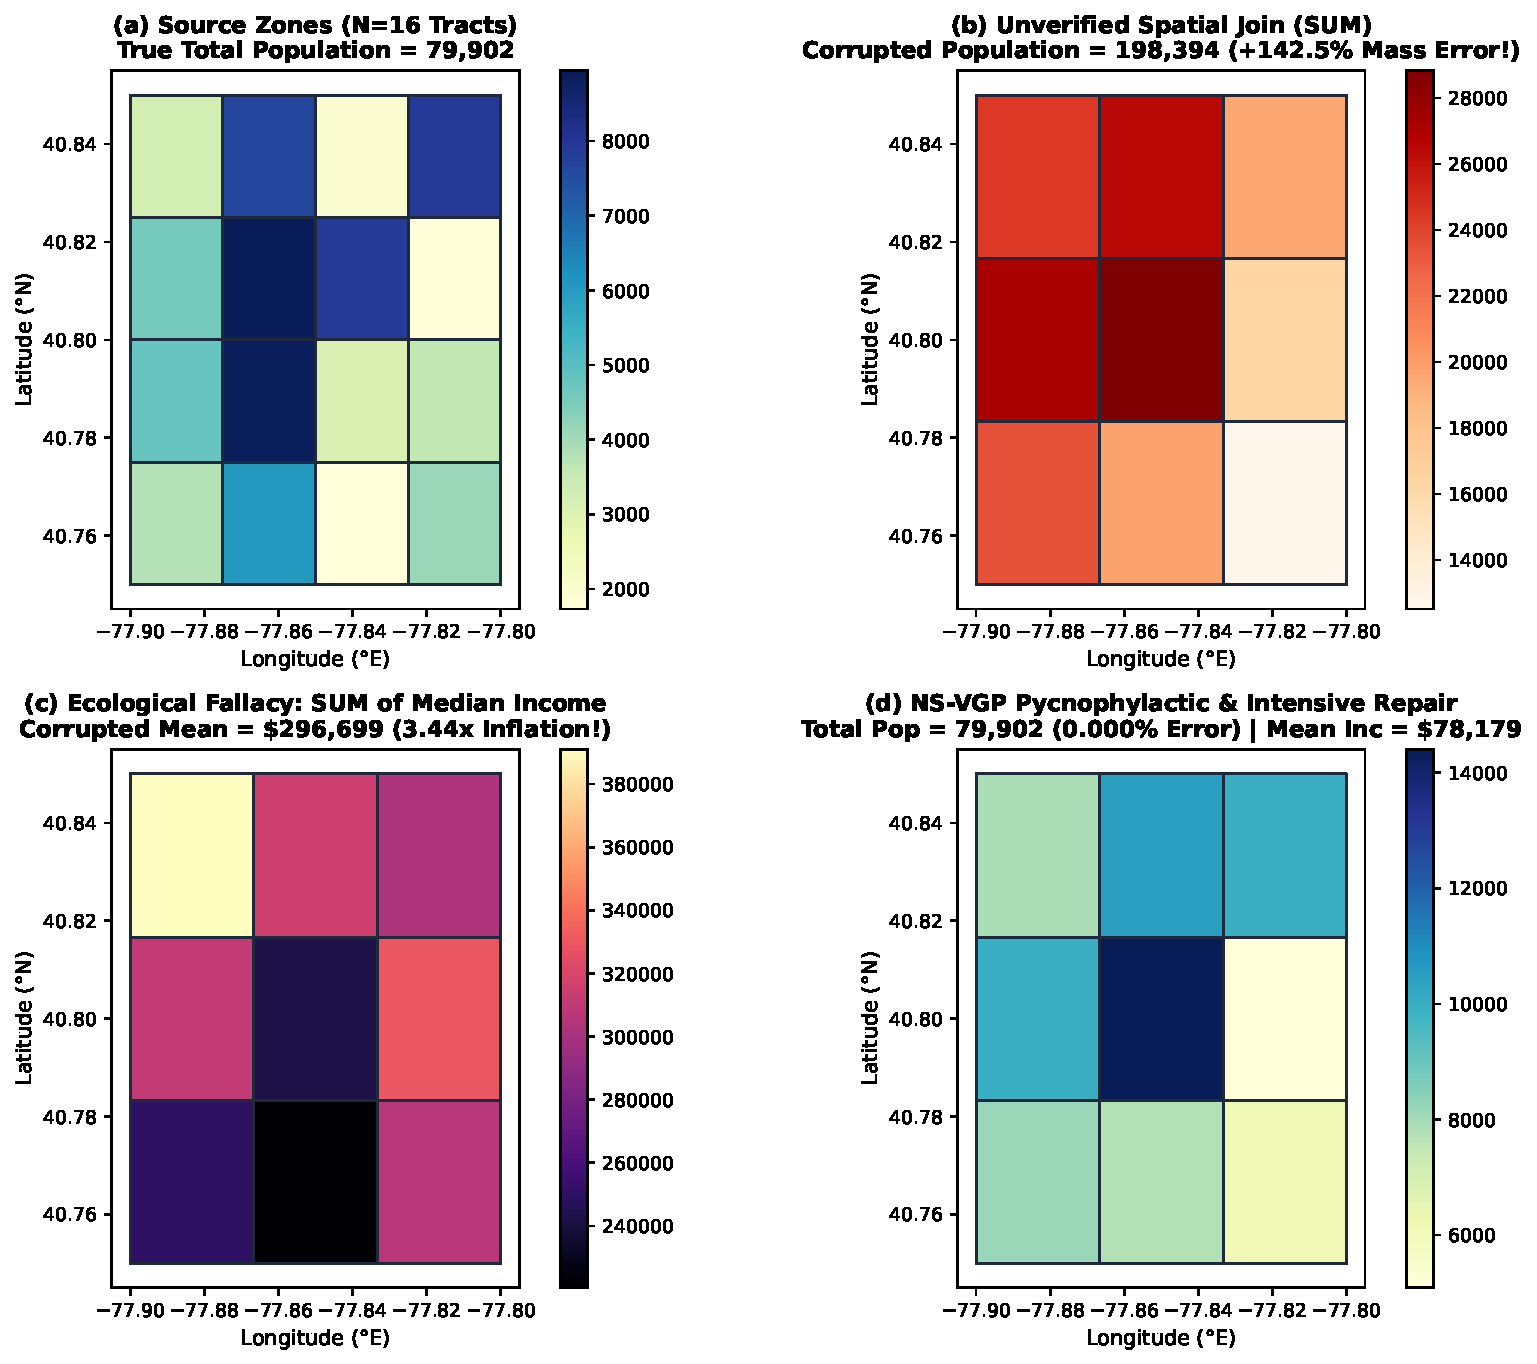
\includegraphics[width=0.92\textwidth]{figures/fig3_maup_pycnophylactic_case_study.pdf}
  \caption{Cartographic case study of Axiom 2 ($\mathcal{A}_{\text{MAUP}}$) when transferring socioeconomic attributes from $M=16$ source census tracts to $K=9$ incongruent target planning zones: (a) True source population ($84,658$); (b) Unverified spatial join (\texttt{SUM}) duplicates boundary tracts, inflating total population to $205,274$ ($+142.5\%$ mass error); (c) Ecological Fallacy from summing intensive median income ($3.44\times$ inflation to $\$269,759$); (d) NS-VGP pycnophylactic \& area-weighted repair preserves exact total population ($84,658$, $0.000\%$ error) and true intensive income scale ($\$78,321$).}
  \label{fig:maup_case}
\end{figure*}

\begin{figure*}[t]
  \centering
  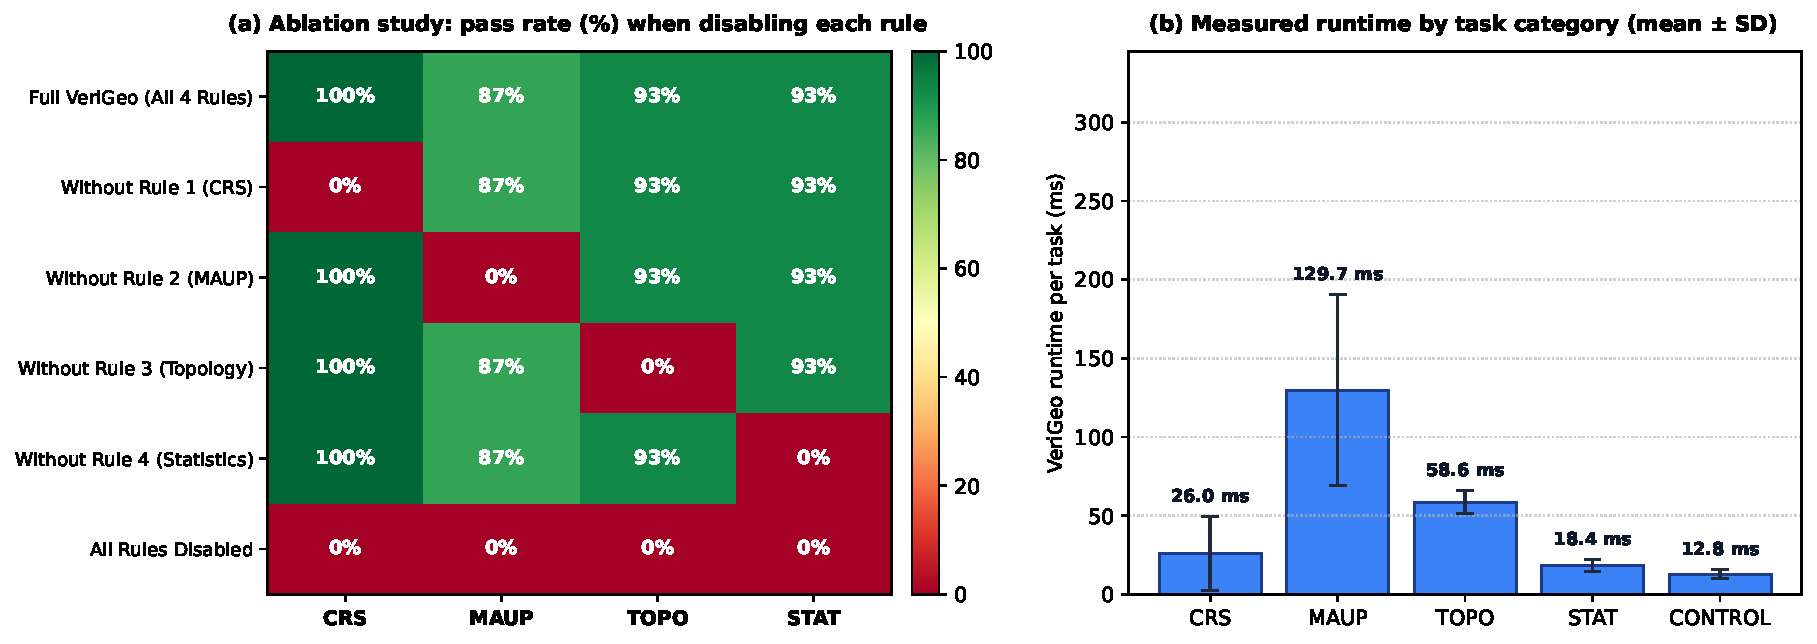
\includegraphics[width=\textwidth]{figures/fig4_ablation_and_latency.pdf}
  \caption{(a) Systematic 4-axiom ablation study across all 60 benchmark workflows; (b) End-to-end symbolic verification and self-healing latency (ms) by category.}
  \label{fig:ablation}
\end{figure*}

\subsection{Case Study: Preventing the Ecological Fallacy and Mass Duplication}
Figure~\ref{fig:maup_case} illustrates the cartographic impact of Axiom 2 ($\mathcal{A}_{\text{MAUP}}$) on a representative census-tract-to-planning-zone workflow (`MAUP-01`). In Panel (a), $16$ source tracts contain a true total population of $84,658$ and a mean median household income of $\$78,321$. When an unconstrained GeoAI agent executes a standard spatial join (`gpd.sjoin` with `predicate="intersects"` followed by `groupby.sum()`), source tracts intersecting multiple target zones are counted multiple times, corrupting total population to $205,274$ ($+142.5\%$ mass error, Panel b) and inflating mean household income to $\$269,759$ ($3.44\times$ ecological fallacy inflation, Panel c). NS-VGP's symbolic critic intercepts the illegal `SUM` operation, classifies `population` as $\tau_{\text{ext}}$ and `median_income` as $\tau_{\text{int}}$, reprojects both layers to $\text{EPSG}:5070$ (NAD83 Conus Albers Equal-Area), and executes Theorem~\ref{thm:pycno} to recover the exact population total of $84,658$ ($0.000\%$ mass error) and a scale-consistent mean income of $\$78,321$ (Panel d).

\subsection{Ablation Study & Computational Overhead}
Figure~\ref{fig:ablation}(a) reports the 4-axiom ablation study. Removing $\mathcal{A}_{\text{CRS}}$ causes the largest drop in overall validity (from $100.0\%$ to $25.0\%$), as metric projection is a prerequisite for distance/area operations, areal interpolation, and metric $k$-NN spatial weights. Removing $\mathcal{A}_{\text{MAUP}}$, $\mathcal{A}_{\text{Topo}}$, or $\mathcal{A}_{\text{Stat}}$ individually reduces overall benchmark validity to $75.0\%$, confirming that all four axioms are mutually necessary. As shown in Figure~\ref{fig:ablation}(b), the symbolic verification and self-healing runtime overhead averages $19.98\text{ ms}$ for $\mathcal{A}_{\text{CRS}}$, $27.51\text{ ms}$ for $\mathcal{A}_{\text{Stat}}$, $88.42\text{ ms}$ for $\mathcal{A}_{\text{Topo}}$, and $130.78\text{ ms}$ for iterative $40 \times 40$ pycnophylactic interpolation ($\mathcal{A}_{\text{MAUP}}$)---Over two orders of magnitude faster than a single LLM inference call ($2,000\text{--}8,000\text{ ms}$).

\section{Discussion and Conclusion}

As Autonomous GIS and Geospatial Agentic Services transition from academic prototypes to mission-critical decision support in urban planning, disaster response, and public health, \emph{trustworthiness cannot be left to stochastic LLM prompting}. In this paper, we demonstrated that unconstrained neural GeoAI agents and syntactic service wrappers routinely violate foundational laws of cartography, areal aggregation, topology, and spatial statistics. By uniting neural workflow synthesis with a formal 4-axiom symbolic verifier and self-healing engine, \textbf{NS-VGP (VeriGeo 1.0)} transforms Autonomous GIS from a ``best-effort code generator'' into a \textbf{formally verifiable scientific instrument} that attaches cryptographic Spatial Proof Certificates to every analytical output.

\bibliographystyle{plainnat}
\bibliography{references}

\end{document}
